\chapter{Architecture}\label{chap:Algorithms}
% =============================================================================
\section{Architecture}
% =============================================================================
Scholar Plot is data visualization tool that uses HTML5, CSS3 and SVG to render a scholar's accomplishment at a glance. We created a MySQL database to store the mapping between the scholar names and their Google scholar IDs. We also designed and created database tables for NSF/NIH/NASA funding data. The user can search the name of the scholar in a text field. When the user starts to enter the name of the scholar, the names in our database which are similar to the entered name will be listed as a drop down list. We use jQuery and Ajax (asynchronous JavaScript and XML) method to have this feature, which connects to the database to get the list of names. If there are no matching/similar names, the user can also insert her/his Google Scholar ID to the database by one click event.

%Once the scholar's name selected, the user can run the application to see the visual results of the selected scholar's publications and fundings. Scholar Plot connects to the Web server to retrieve the necessary information.
The server-side application is implemented in PHP scripting language and MySQL. The HTTP protocol is used for communicating between client-side and server-side to get the basic information via JSON format (JavaScript Object Notation) and JSONP function (Figure \ref{fig:fig-arch}). Scholar Plot also uses htmlSQL library to parse Google scholar's page to extract user basic information \cite{htmlSQL}.
%, collecting for the publication title, the journal name, the co-authors' name, the year, and the citations. It also collects the {\it h-}index and the number of total citations from the top of the scholar's page up to 300 publications.

\begin{figure}
\centering
  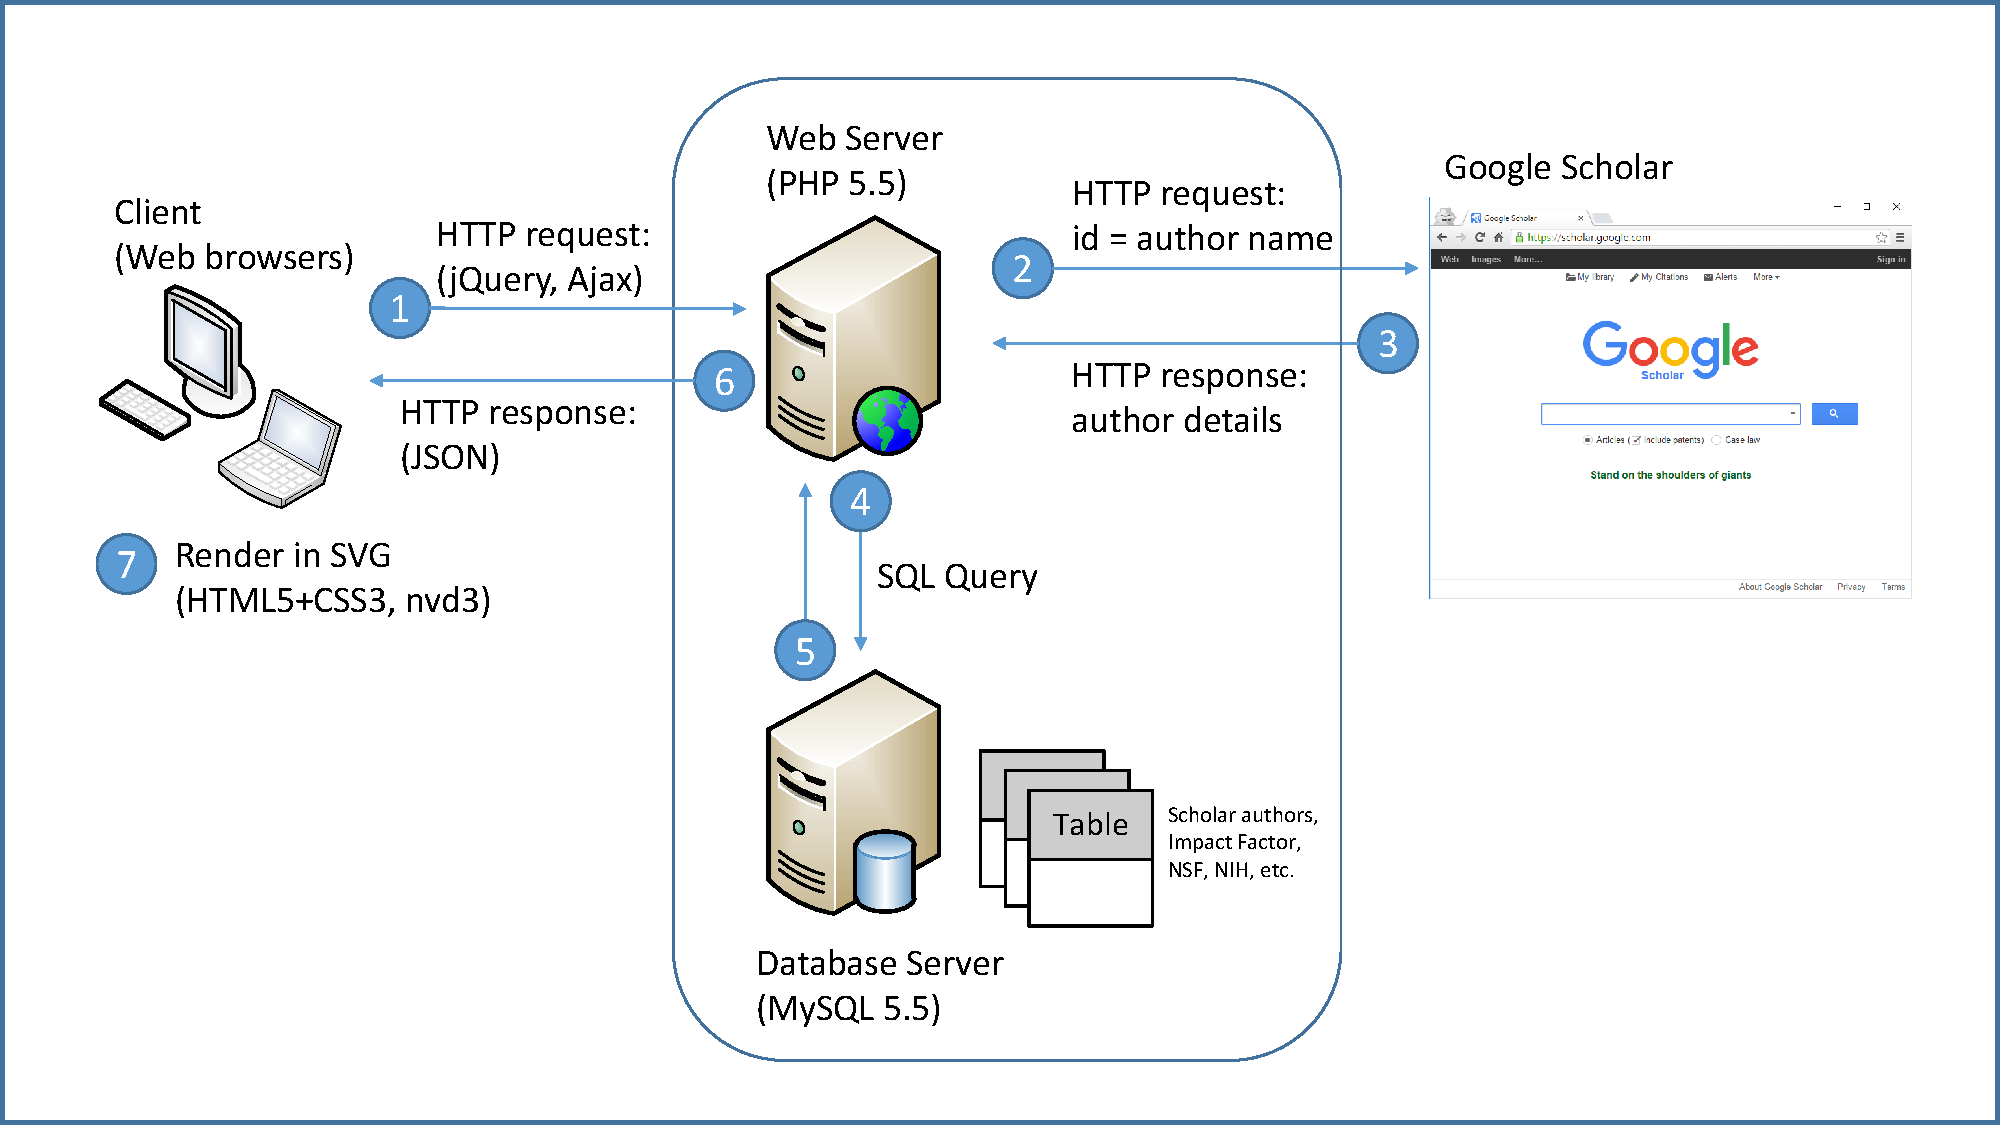
\includegraphics[width=1\columnwidth]{figures/fig_system_architecture.pdf}
  \caption{System Architecture of Scholar Plot.}~\label{fig:fig-arch}
%\vspace{-1ex} 
\end{figure}

The NSF/NIH/NASA funding datasets are available at the respective US government websites in various file formats such as XML, CSV and so on \cite{nsf, nih}. We implemented a script to parse this massive XML dataset into our data structure that consists of AwardID, AwardAmount, First name, Last name, Investigator by RoleCode (Principal Investigator, Co-Principal Investigator and Former Principal Investigator), using XMLStarlet \cite{XMLStarlet}. We imported this data to our database using Toad DBMS tool.

% =============================================================================
\section{Database Schema Diagrams}
% =============================================================================
\begin{figure}
\centering
  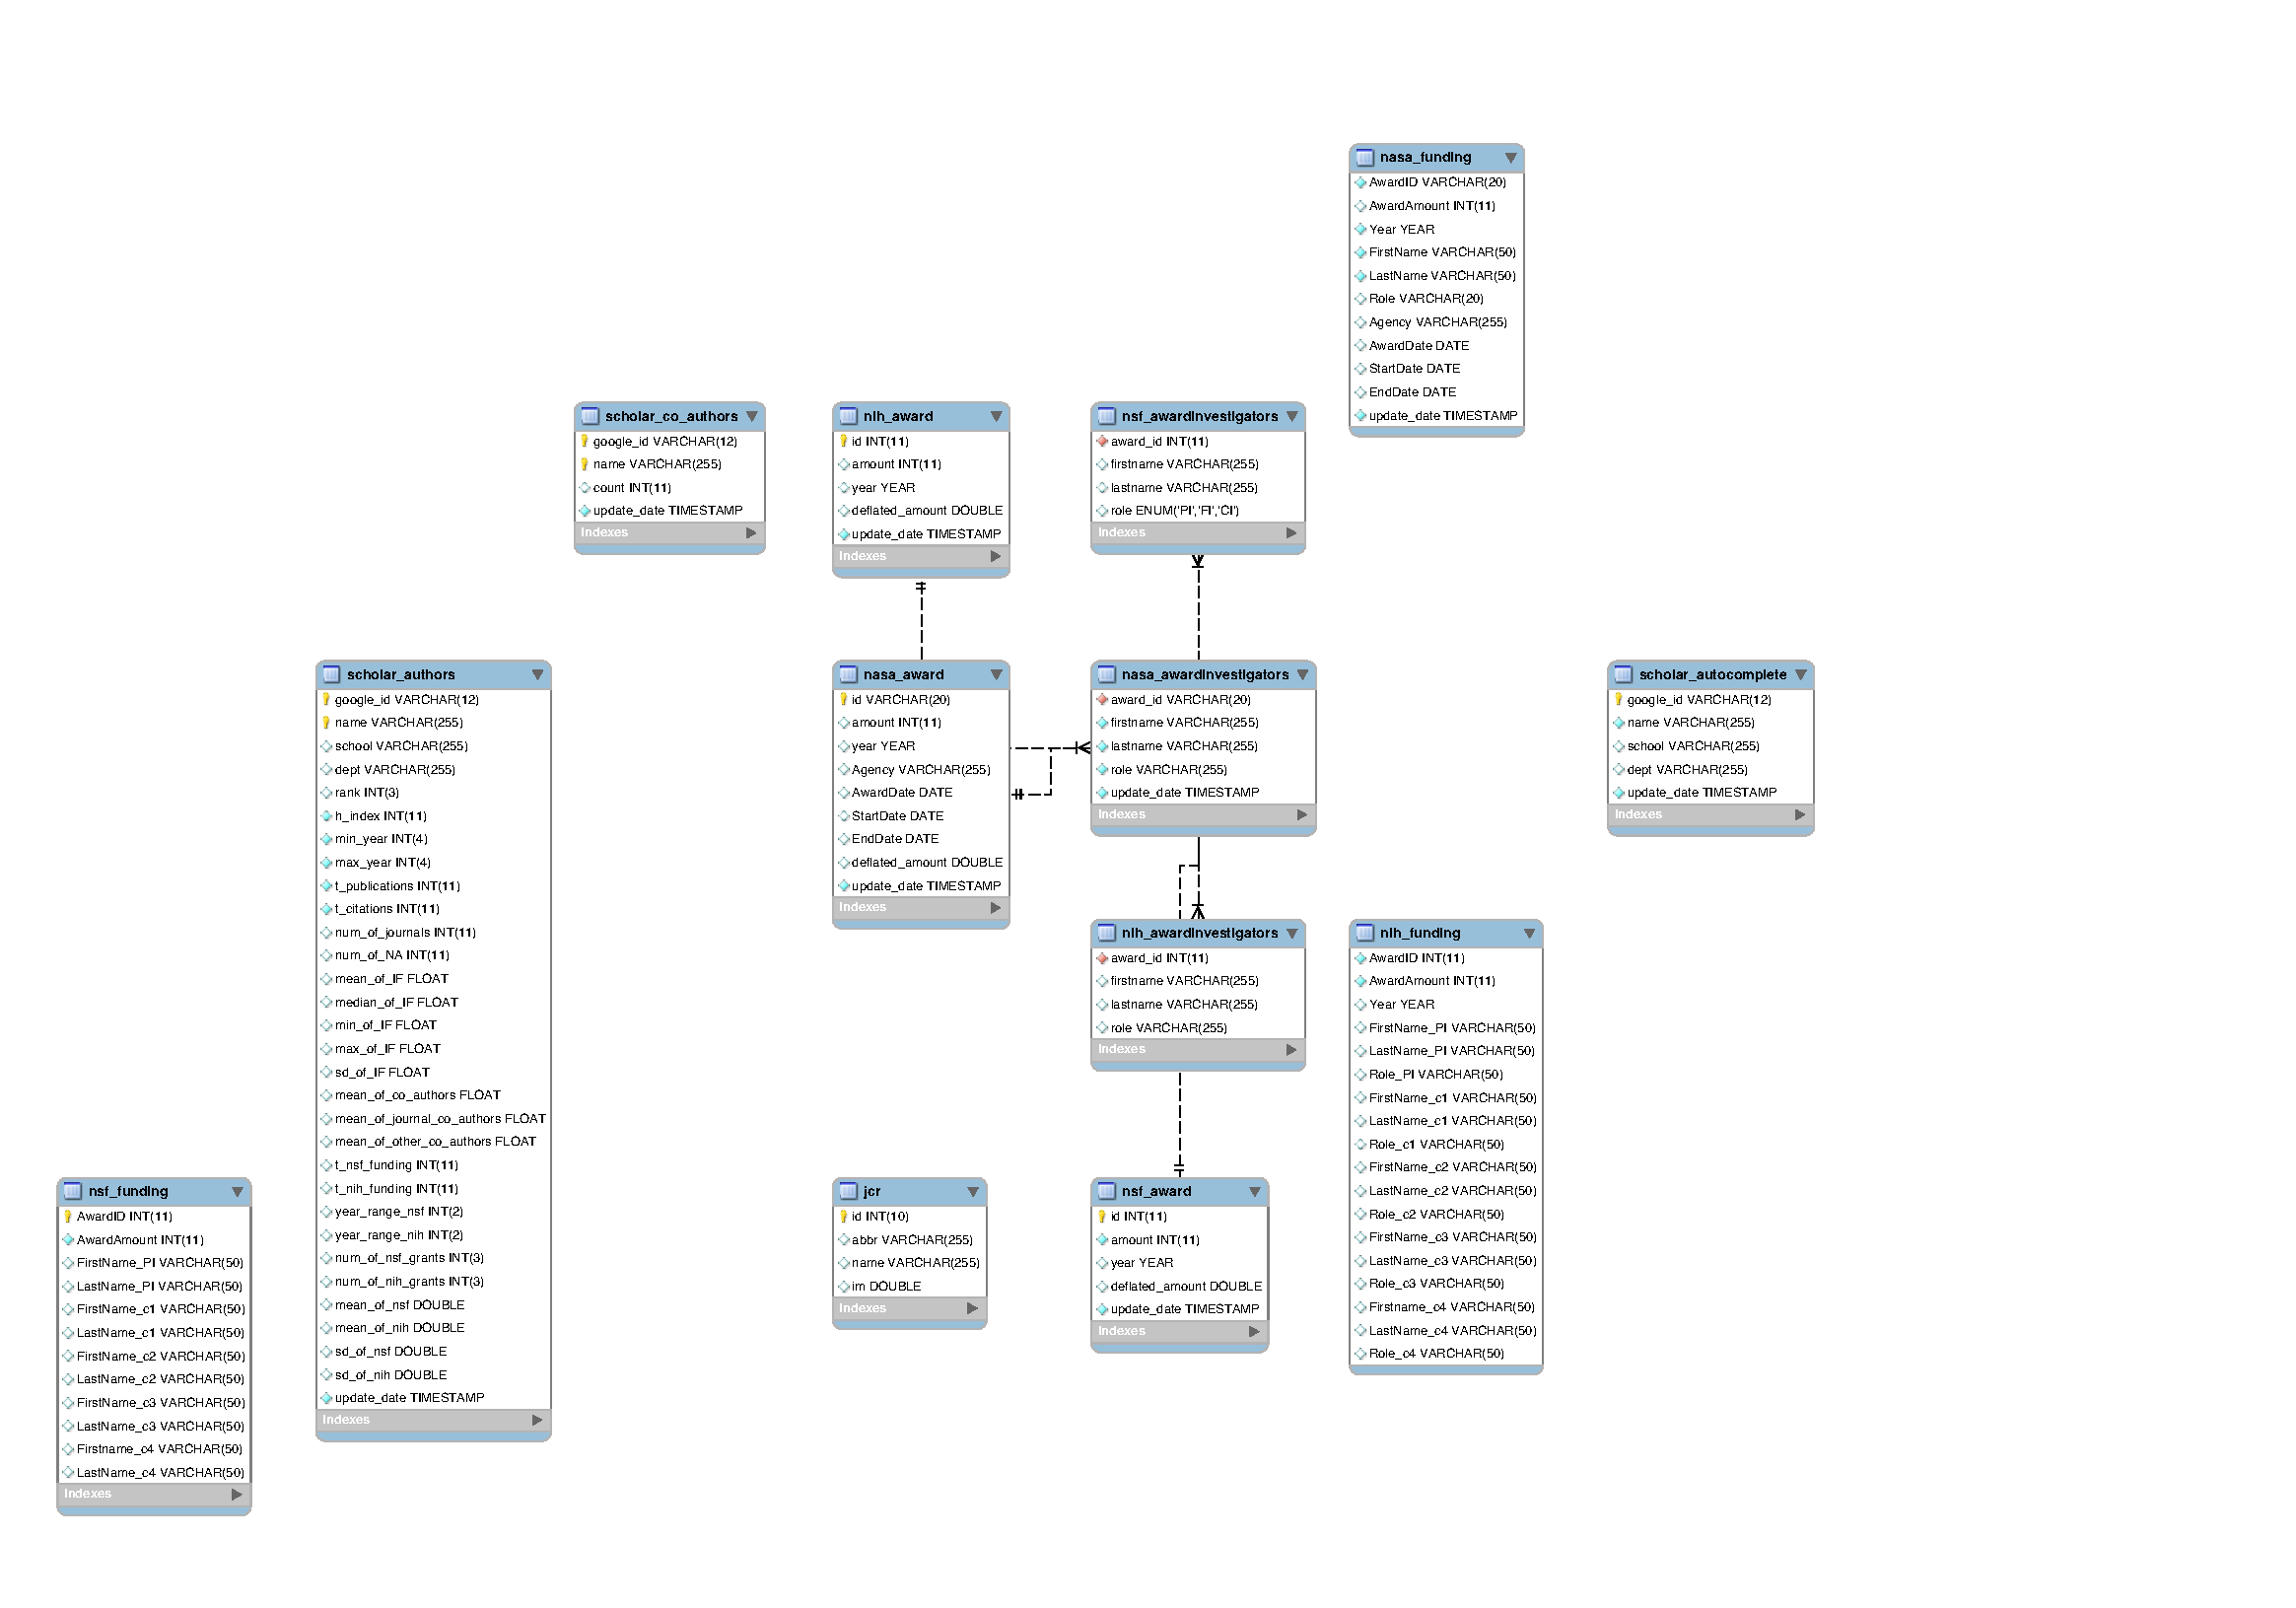
\includegraphics[width=1\columnwidth]{figures/fig_EER_Diagram.pdf}
  \caption{System Architecture of Scholar Plot.}~\label{fig:fig-arch}
%\vspace{-1ex} 
\end{figure}





% =============================================================================
\section{Name Disambiguation}
% =============================================================================
Google Scholar data has to be cleaned because it contains many non-english characters. We use regular expression to remove the invalid special characters and translate phonetic characters to english alphabets. We designed and implemented Algorithm to match the author names in Google Scholar with those in NSF/NIH/NASA data. This process helps to improve the quality of results. 




% =============================================================================
\section{Name Disambiguation - Details}
\subsection{Within and across profile author name disambiguation}

Let $i$ be an index for the Google scholar profile researchers. Within each collaboration profile of $i$,  there are a set of $K_{0}$ raw name strings that you have extracted,  $Names_{k}$ indexed by $k_{i}$. We will use the fact that these strings are associated with profile $i$ in the process of name disambiguation across Google Scholar profiles. The following provides an outline of this procedure: \\


A) {\bf Clean last names:} 
Remove strings at end of all $Names_{k}$ that are not last names, and which may not consistently be listed for $k$, e.g. ``Jr.'', ``III'' etc. Hence, each name string  $Name_{k}$ consists ideally of a First name string $FN_{k}$, a Last name string $LN_{k}$, and possibly a Middle name string $MN_{k}$. \\

B)  {\bf Clean middle initial strings within each profile $i$:}  Within each $i$, search for inconsistencies in the use of $MN_{k}$. That is, possibly sometimes the author $k$ is listed as {\it Alexander M Petersen}, sometimes {\it Alexander Petersen}, and sometimes {\it Alexander Michael Petersen}. In this example the Last name string $LN_{k} = Petersen$ and the First name string $FN_{k} = Alexander$ are clearly consistent. But the Middle name string \{$\_$ , M, Michael\} causes some ambiguity if simple string comparison is used,  where $\_$ is a whitespace. 

%Hence, for each distinct  surname $FN_{k}$ and last name $LN_{k}$, map all $MN_{k}$ strings to the simplest representation $\hat X$ of just the middle name initials.\\

Then check to see how many different types of {\it Alexander} $\hat X$ {\it Petersen} occur within each $k$, where $\hat X$ is refers to the middle name. Use the following rules for when there are 2 or more types of $\hat W \hat X Petersen$.
 
 \begin{itemize}
 \item If there are only two  types of $Alexander \hat X Petersen$, with $\hat X=$ $\_$ or $M$, then map all of the $Alexander \hat X Petersen$ to $Alexander M Petersen$ for this $i$
 \item If there are only three types of $Alexander \hat X Petersen$, with $\hat X=$ starting with the same initial, $M\_$ or $M$, then map all of the $A\hat X Petersen$ to $Alexander Michael Petersen$ for this $i$
 \item If there are two or more types of $Alexander \hat X Petersen$, say $\hat X=O$ and $\hat X=P$, then keep these $X$ as they are.
 
%  \item However, if one of those types are a whitespace,  say $\hat X=O$ and $\hat X=P$  and $X= \_$, then we cannot know if the latter possibly corresponds to $O$ or $P$. This case shouldn't occur often. So we can use the simple heuristic that if there is any paper with $AO$ and $A$, then in this case the latter is actually $AP$, and so all $A\_$ are mapped to $AP$. If there are no papers that make obvious this distinction,  then compare the coauthors of $AO$ and $AP$  and $A \_$ within the profile of $i$. Map $A \_$ to $AP$ if they share more coauthors or map $A \_$ to $AP$ if they share more coauthors using the Jaccard Similarity measure to compare.
  
\end{itemize}

C)  {\bf Disambiguate coauthors $k$ across the Google Scholar profiles (connecting $i$):} Let  $k$ and $k'$ be coauthors in profiles $i$ and $i'$, respectively.   In this step we would like to identify $k$ and $k'$ that are likely the same person, $k=k'$, allowing us to connect the two profiles $i$ and $i'$ within the coauthor network.\\

 If $k$ and $k'$ have the same initials and same surname, then there is a possibility that they are the same individual. Also, if their full first name strings match, this is clearly very positive evidence of this. Let $A_{k,j}$ be the entire combination of First Name and Middle initial $FM_{k,j}$ with the surname $L_{k,j}$ (e.g. {\it Adam B Smith}, or {\it Adam \_ Johnson}) of the coauthor $j$ of the coauthor $k$. 

 \begin{itemize}
 \item If the full first name strings and the full last name strings are the same, $FN_{k,j}$=$FN_{k',j}$ and $LN_{k,j} = LN_{k',j}$ (e.g. Adam J. Johnson and Adam Johnson), and they both have at least one coauthors in common,  then they are considered the same coauthor. 
 \item If we don't have the added information of their full first names then we must rely more heavily on the information from their coauthors. If the first and last names are the same, $FM_{k,j}=FM_{k',j}$ and $LM_{k,j}=LM_{k',j}$, and there are more than 2 middle names with one of the middle name being empty, we do the following -
 
 We compute the number of coauthors in common of the empty middle name author with non-empty middle name authors by comparing the sets of coauthors, $\{j\}$.% and $\{j'\}$.
 
 We assign the empty middle name to that middle name for which there are more number of co-authors in common.
 
 \item If the first name of the author has a hyphen, we check for any other author having the same last name and the first name as the first word of the hyphenated word and middle name starting with the first letter of the second part of the hyphenated word. If any such pair of authors have at least one author in common, we update the first and middle name of the author with the hyphenated middle name to first name and middle name of the matched author.


\item If the first name of the author has only two letters, we check for any other author having the same last name and the first name starting with the first letter of the first name and middle name starting with the second letter of the first name. If any such pair of authors have at least one author in common, we update the first and middle names of the author with two letters to first and middle names of the matched author.
  
\end{itemize}
Google Scholar data has to be cleaned because it contains many non-english characters. We use regular expression to remove the invalid special characters and translate phonetic characters to english alphabets. We designed and implemented Algorithm \ref{alg:name} to match the author names in Google Scholar with those in NSF/NIH/NASA data. This process helps to improve the quality of results. 


%% =============================================================================
%\section{Scholar Plot Design - Base Level}
%% =============================================================================
%The base level of Scholar Plot (SP) visualizes individual academic records. The first issue we had to address as part of the design process for this level was to determine what to visualize. To answer this question we looked at the merit criteria considered by promotion, tenure, and search committees; these are: a) publication quality and quantity, and b) research funding. Furthermore, publication quality is defined by two factors: citation counts and prestige of the journals where the publications appeared. 
%
%Accordingly, we decided to structure individual scholar plots as two-panel arrangements - the top panel visualizing the individual's publication record, while the bottom panel visualizing the individual's research funding record (Fig. \ref{fig:ScholarPlot}). This arrangement brings to the fore any causal relationship that may exist between funding and publishing, as publication production is often powered by research dollars. The common timeline in the horizontal axes of the two panel graphs facilitates such an association. 
%
%\begin{figure*}
%%  \begin{minipage}{\columnwidth}
%    \centering
%    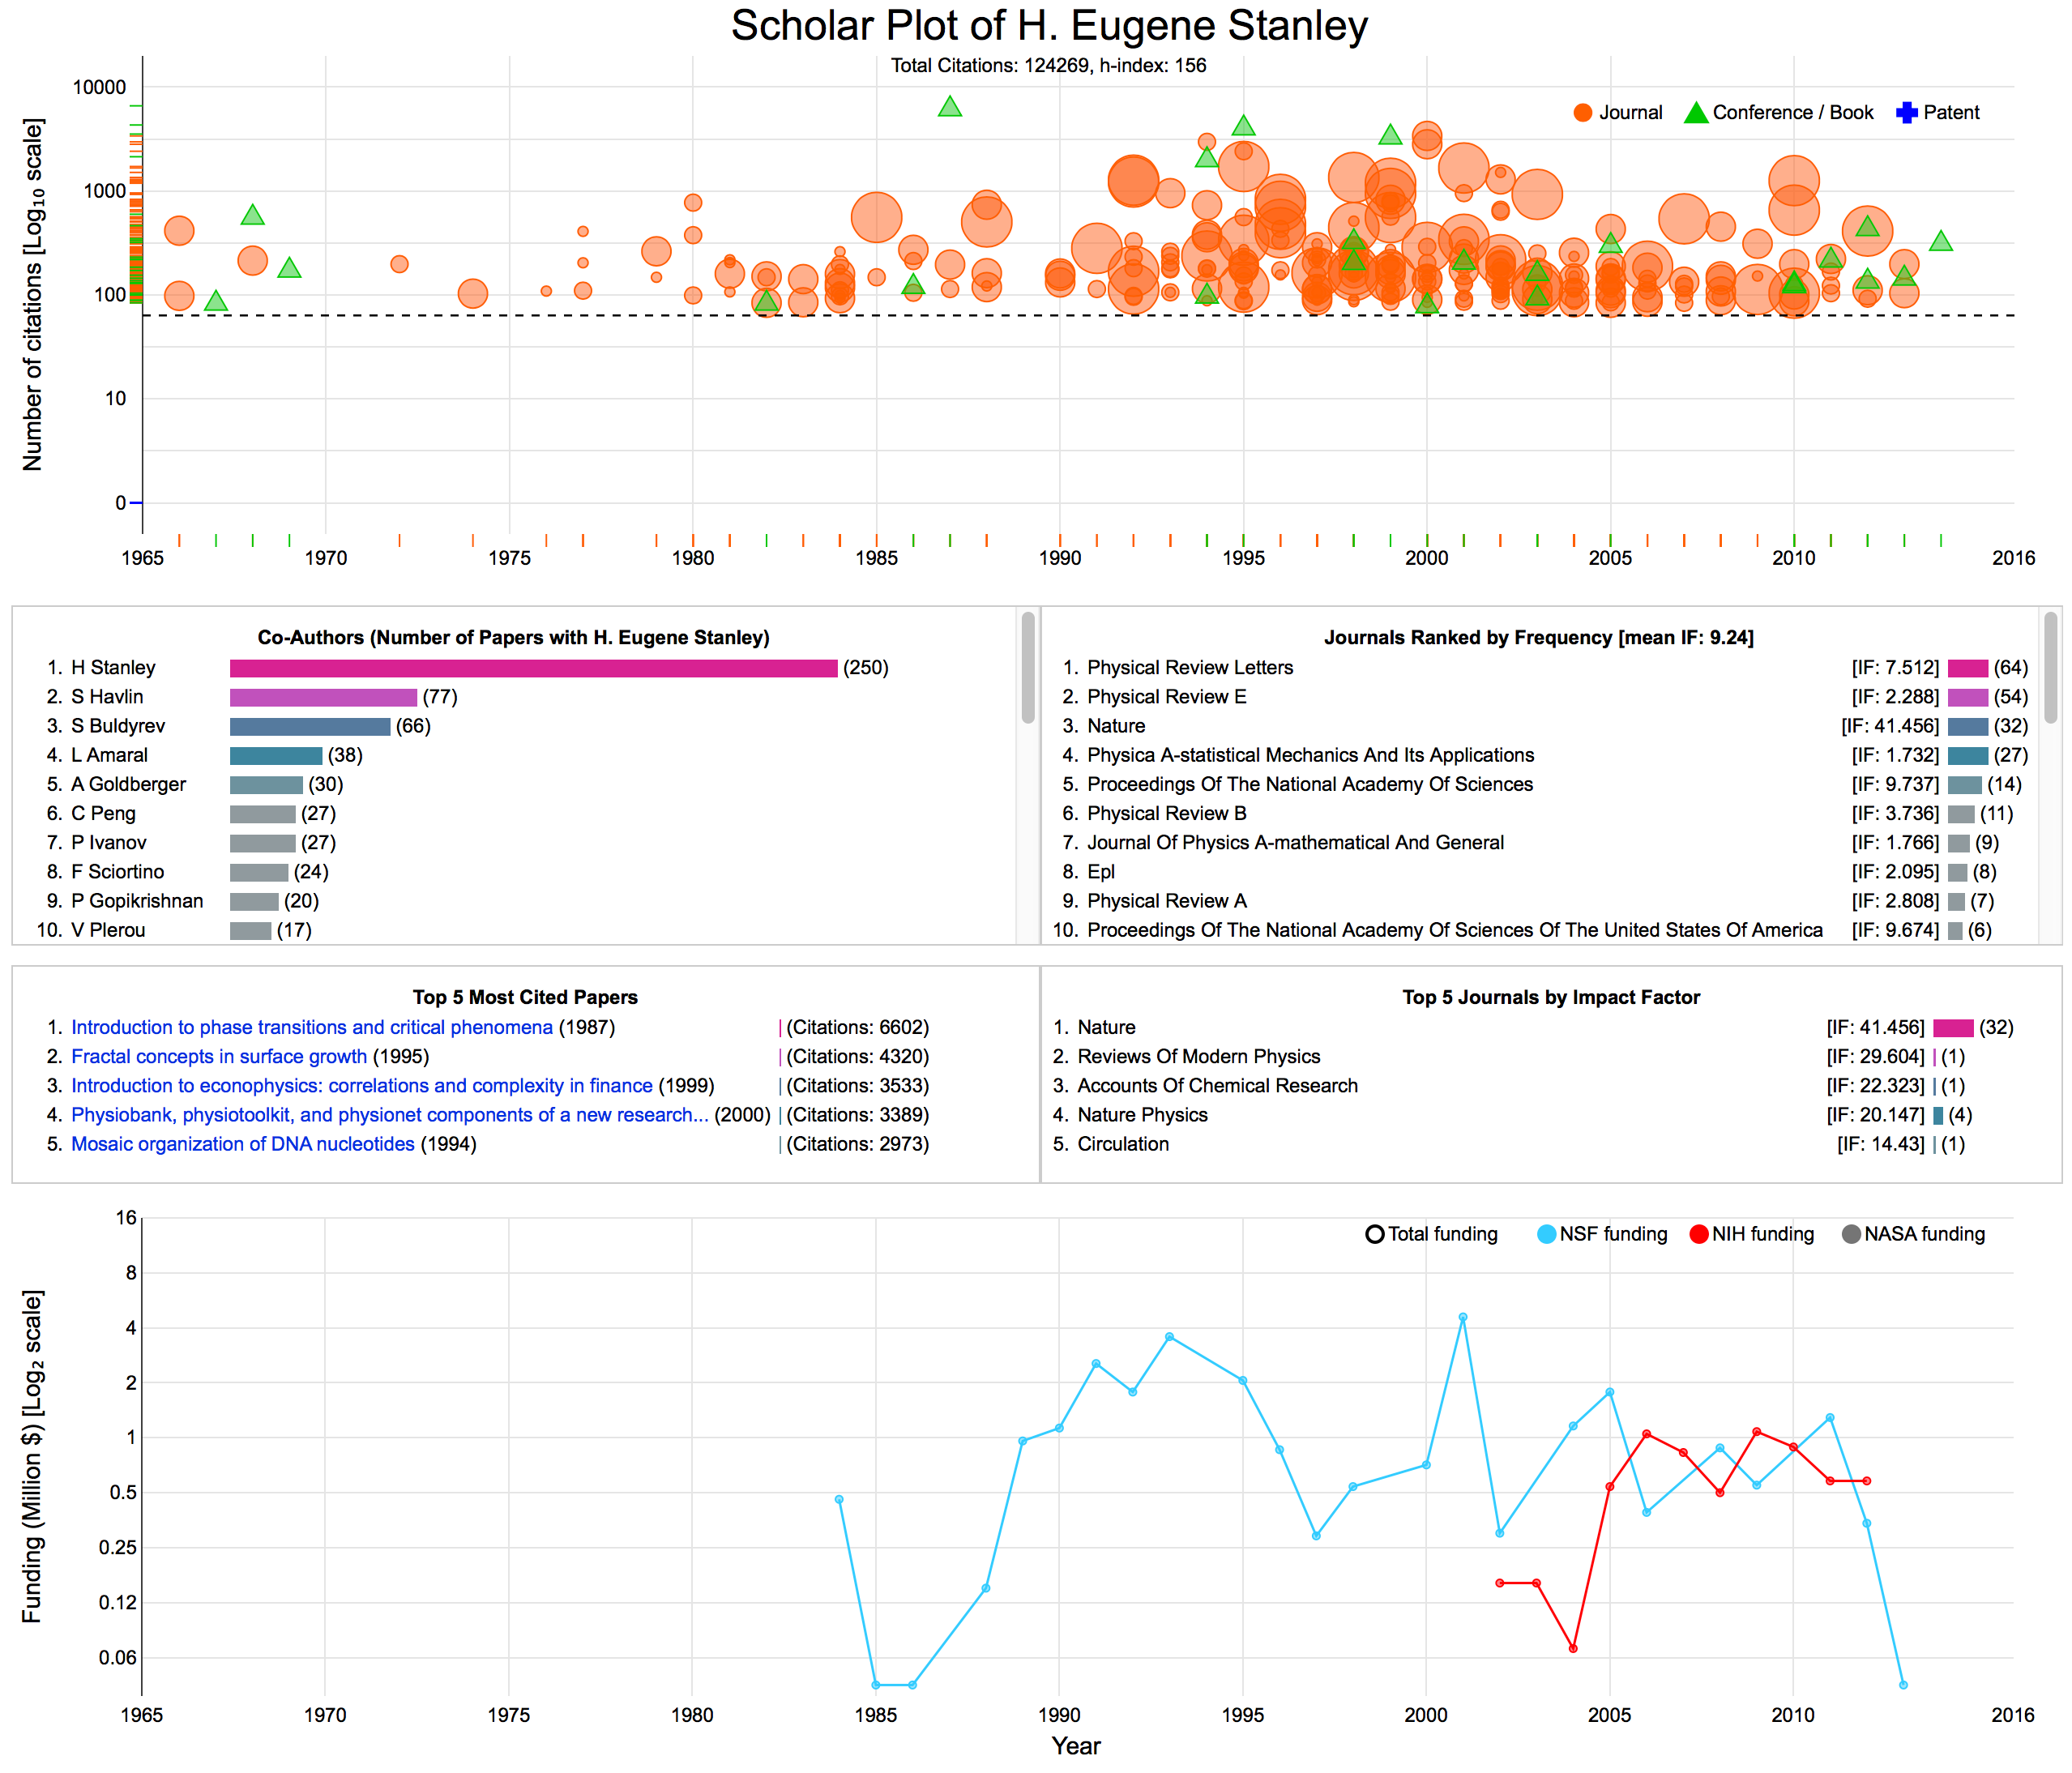
\includegraphics[width=1\textwidth]{figures/fig-EugeneStanley}
%    \caption{Base level Scholar Plot (SP) example - a famous physicist and interdisciplinary scientist with dozen of articles in \emph{Nature}. The summary panels in the middle were added after feedback from the focus group. Notice how this scholar's publication production exploded in sync with the commencement of substantial federal funding.}~\label{fig:ScholarPlot} 
%%    \end{minipage}
%\end{figure*} 
%
%The vertical axis of the publication graph indexes citation counts (Fig. \ref{fig:ScholarPlot}) - an important quality indicator for a publication. As we mentioned, the prestige of the publication venue is another important quality indicator. We convey this additional measurement dimension by varying the size of the graph points. 
%
%Only journals have a widely accepted ranking system reflecting prestige - the Journal Impact Factor (IF) List, issued every year by Thomson Reuters. Hence, we opted to represent different publication types with different symbols,  varying the symbol size of  journal publications only, for which an established ranking system exists. We chose disks to be the symbols of journal publications, as disk scaling can be done very effectively by simply varying its radius ($A \sim r^2$). Specifically, after performing histogram analysis on the IFs of journal publications, we settled on four disk sizes to represent journal prestige: $\#1 < \#2 < \#3 < \#4$ (Fig. \ref{fig:symbols}). We found that the great majority of journal publications appear in journals with $\mbox{IF} < 2$, assigning to this cohort the smallest disk size symbol, $\# 1$.  These are mid-level specialized technical and scientific journals. The next IF bracket  ($2 \leq \mbox{IF} < 4$) includes high quality specialized technical (e.g., IEEE Transactions) and scientific journals represented by disk \#2. The third IF bracket ($4 \leq \mbox{IF} < 16$) includes  very high quality science journals and specialized medical journals represented by disk  \#3. The top IF bracket ($\mbox{IF} \geq 16$) includes famous general science journals (e.g., \emph{Nature}) and top medical journals (e.g., \emph{New England Journal of Medicine}); they are assigned the largest disk, $\#4$.
%
%In the funding graph, each funding agency is represented by a polyline with a characteristic color (Fig. \ref{fig:ScholarPlot}). Grants are reported at the year they were awarded. If more than one grant was awarded by the same agency the same year to the specific investigator, then the full list shows up by rolling the mouse over the corresponding point in the polyline.
%
%The end effect of this simple visualization scheme is a picture that does not only compress dozens of CV pages, but also brings to the fore nuanced information about an academic's profile that can be grasped at a glance. Here are some examples:
%\begin{figure*}
%%  \begin{minipage}{\columnwidth}
%    \centering
%    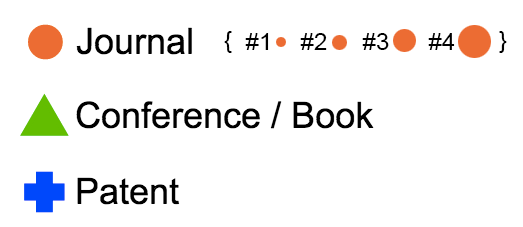
\includegraphics[width=0.5\textwidth]{figures/fig-disksize}
%    \caption{Publication symbols.}
%    \label{fig:symbols} 
%%    \end{minipage}
%\end{figure*}
%\begin{enumerate}
%\item It is easy to identify what type of publication powers the individual's scholarship - a correlate of disciplinary culture. For example, it is easy to spot career profiles of computer scientists and engineers (Fig. \ref{fig:Splots}a), where typically scholarship is built on conference rather than journal publications.
%\item It is easy to identify if the individual's scholarship is heavily associated with high or mid/low IF journals. If the publication graph is full of mid or small disks, this indicates that the scholar has done prolific methodological work that appeared in good specialized journals (Fig. \ref{fig:Splots}b). If the publication graph is full of large disks, this indicates that the scholar has done trendy and novel work that appeared in famous journals (Fig. \ref{fig:Splots}c).
%\item It is easy to identify if high funding levels yield high quantity and quality of publications or not (Fig. \ref{fig:ScholarPlot}). This may be especially useful to NSF and NIH reviewers who assess among other things the quality and impact of the investigator's prior work for the funding amounts s/he received.
%\begin{figure*}
%    \centering
%    \subfigure[SP of an accomplished Engineer.]{%
%    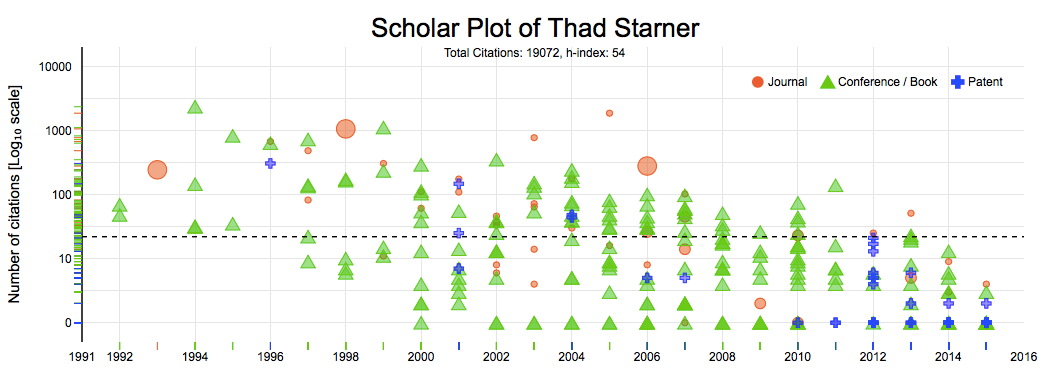
\includegraphics[width=1.0\textwidth]{figures/fig-ThadStarner}
%    } \\
%    \subfigure[SP of an accomplished Physicist.]{%
%     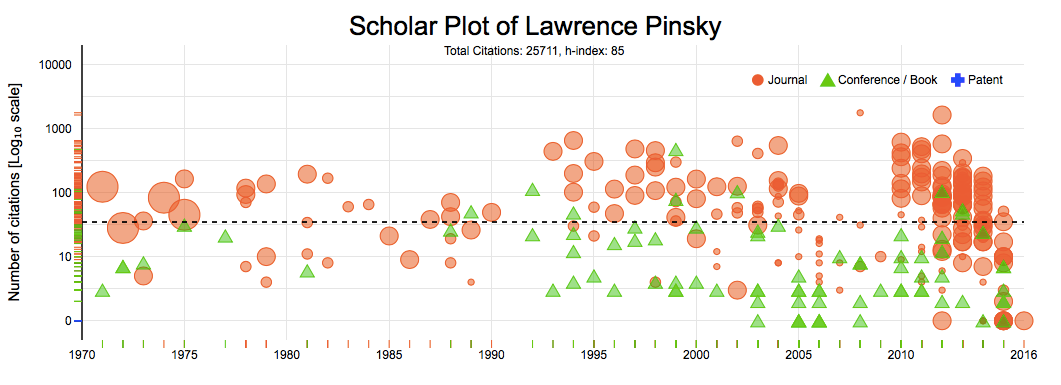
\includegraphics[width=1.0\textwidth]{figures/fig-LawrencePinsky}
%     }\\
%      \subfigure[SP of a famous Interdisciplinarian.]{%
%     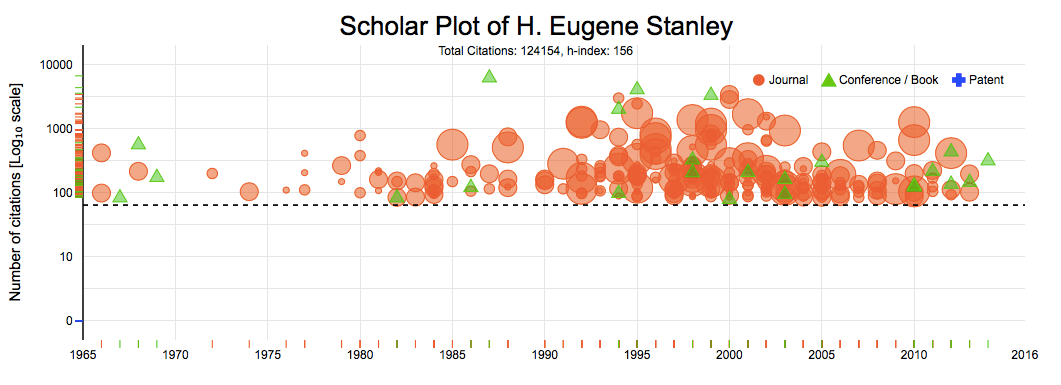
\includegraphics[width=1.0\textwidth]{figures/fig-EugeneStanley-pub}
%     }
%     \caption{}~\label{fig:Splots} 
%\end{figure*} 
%\end{enumerate}
%
%% =============================================================================
%\section{Scholar Plot Data Sources}
%% =============================================================================
%There were several options to get bibliographic data for powering the publication graph of Scholar Plot (SP). These included \href{http://www.scopus.com/}{Scopus}, \href{http://www.isiknowledge.com/}{ISI Web of Knowledge}, and \href{http://scholar.google.com}{Google Scholar}. We chose Google Scholar for two reasons: a) it is all inclusive, covering all types of publications, that is, journals, conferences, books, and patents; and, b) it is freely available.
%
%Our choice carries a few challenges, too. Google Scholar does not provide an application programming interface. Hence, we had to develop elaborate software to scrape information off publicly available Google Scholar pages. Also, not every academic has a Google Scholar page. This has been changing fast, however, as one college after the other in the United States mandating their faculty to maintain a Google Scholar page. 
%
%We use the Journal IF List issued every year by Thompson Reuters to assign disk sizes to journal publications.
%
%For funding records, we use the publicly available grant records from the \href{http://www.nsf.gov/awardsearch/download.jsp}{National Science Foundation (NSF)}, the \href{http://exporter.nih.gov/ExPORTER_Catalog.aspx}{National Institutes of Health (NIH)}, and the \href{https://www.research.gov/research-portal/appmanager/base/desktop?_nfpb=true&_eventName=viewQuickSearchFormEvent_so_rsr}{National Aeronautics and Space Administration (NASA)}. These are the only funding agencies with publicly available datasets at this point.
